
The $Z+$jets background has a very different $E_{\text{T}}^{\text{miss}}$ signature than VBF as this sample does not contain the level expected from VBF Higgs events. Thus a BDT trained to discriminate between VBF signal events and the $Z+$jets background uses a range of $E_{\text{T}}^{\text{miss}}$ variables and cutting on this trained discriminant rather directly on $E_{\text{T}}^{\text{miss}}$ provides an enhanced purity. The training and results from the BDT are described in the next subsection. Note that the following results from substantial obtimization on training inputs and techniques where the final BDT has high discrimination, no under or overtraining, and utilizes variables which are well-modelled and not highly correlated to one another.  

A decision tree is a collection of cuts designed to classify events as signal-like or background-like. A given signal event is correctly identified if it is placed in a signal-dominated leaf and vice-cersa for background events. After the initial tree is built another tree is grown to better separate the signal and background events misidentified by the first tree. This proceeds iteratively until there is a collection of a specified number of trees, in a process known as boosting. A weighted average is taken from all these trees to form a BDT output discriminant with values ranging from -1 to 1.

The BDT is trained using $e\mu+\mu e$ events after the VBF selection and the signal regions cuts including that on $n_{jets}$, $b$-veto, OLV, CJV, $M_{jj}$ and $DY_{jj}$. In this way, the phase space in which we train the BDT is exactly the same as the one where we apply it. The training includes only the $Z\rightarrow\tau\tau$ background and the VBF signal. The MC statistics used in the training are half those available after all signal region cuts (as the other half are later used to test the training). This corresponds to $\approx$ 5,000 $Z\tau\tau$ events and $\approx$100,000 VBF events.

The TMVA BDTG interface is used to train and test the BDT. The optimal parameters were found through a scan of reasonable values and the final set is summarized in Table~\ref{tab:ZBDTparameters}.

\begin{table}[htbp!]
\centering
\begin{tabular}{|l|c|c|}
\hline
Parameter                                    & Value    & Range     \\
\hline
Boosting algorithm                           & Gradient & --        \\
Maximum tree depth                           &  22      & [3,10,22,30]    \\
Number of trees                              &  1000    & [200,1000,10000] \\
Minimum number of events requires per mode   &  5\%     & [5\%]\\
Number of cuts                               &  7       & [3,5,7,9]  \\
\hline
\end{tabular}
\caption{BDT parameters used for the $Z\rightarrow\tau\tau$ training.} 
\label{tab:ZBDTparameters}
\end{table}

For this BDT we aim to take advantage of the different $E_{\text{T}}^{\text{miss}}$ distributions in $Z\rightarrow\tau\tau$ backgrounds and VBF signal Monte Carlo events. Instead of a cut on $E_{\text{T}}^{\text{miss}}$, we train the BDT using multiple different $E_{\text{T}}^{\text{miss}}$ variables to maximize discrimination and then cut on the BDT output variable. Training using variables including $E_{\text{T}}^{\text{miss}}$, $\ensuremath{E_{\text{T}}^{\text{miss, track}}}$, $\ensuremath{E_{\text{T,rel}}^{\text{miss}}}$, $\ensuremath{E_{\text{T,rel}}^{\text{miss, track}}}$, $\Delta\phi_{\ell\ell,E_{\text{T}}^{\text{miss}}}$, $\Delta\phi_{\ell\ell,E_{\text{T}}^{\text{miss, track}}}$, and $\ensuremath{E_{\text{T}}^{\text{miss, significance}}}$ have been tested. The optimal analysis uses $\ensuremath{E_{\text{T}}^{\text{miss, significance}}}$, $\ensuremath{E_{\text{T}}^{\text{miss, track}}}$, $\ensuremath{E_{\text{T,rel}}^{\text{miss}}}$, and $\ensuremath{E_{\text{T,rel}}^{\text{miss, track}}}$, $\ensuremath{\Delta\phi_{\ell\ell,E_{\text{T}}^{\text{miss, track}}}}$, and $\ensuremath{\Delta\phi_{\ell\ell,E_{\text{T}}^{\text{miss}}}}$. Relative $E_{\text{T}}^{\text{miss}}$ is defined as $E_{\text{T}}^{\text{miss}} * \sin(|\Phi_{E_{\text{T}}^{\text{miss}}}\Phi_{jet}|)$, $\ensuremath{E_{\text{T}}^{\text{miss, track}}}$ is calculated from tracking detectors while $E_{\text{T}}^{\text{miss}}$ is calculated from calorimeter deposits. Finally, $\ensuremath{E_{\text{T}}^{\text{miss, significance}}}$ is a newly calibrated variable from the Jet/$E_{\text{T}}^{\text{miss}}$ group that differentiates between $E_{\text{T}}^{\text{miss}}$ from electroweak and strong interactions \cite{JETEtmiss}. While $\ensuremath{E_{\text{T}}^{\text{miss, significance}}}$ wasn't shown to increase the discrimination of the BDT due to its high correlations with $E_{\text{T}}^{\text{miss}}$, replacing this variable with $E_{\text{T}}^{\text{miss}}$ showed very similar results while reducing correlations between variables like $\ensuremath{E_{\text{T,rel}}^{\text{miss}}}$ and $\ensuremath{\Delta\phi_{\ell\ell,E_{\text{T}}^{\text{miss}}}}$. Plots shown in \ref{fig:ZjetsBDTinput} and \ref{fig:ZjetscorrSB} demonstrate the input distributions used to train the BDT and their correlations.

\begin{figure}[!htbp]
    \centering
    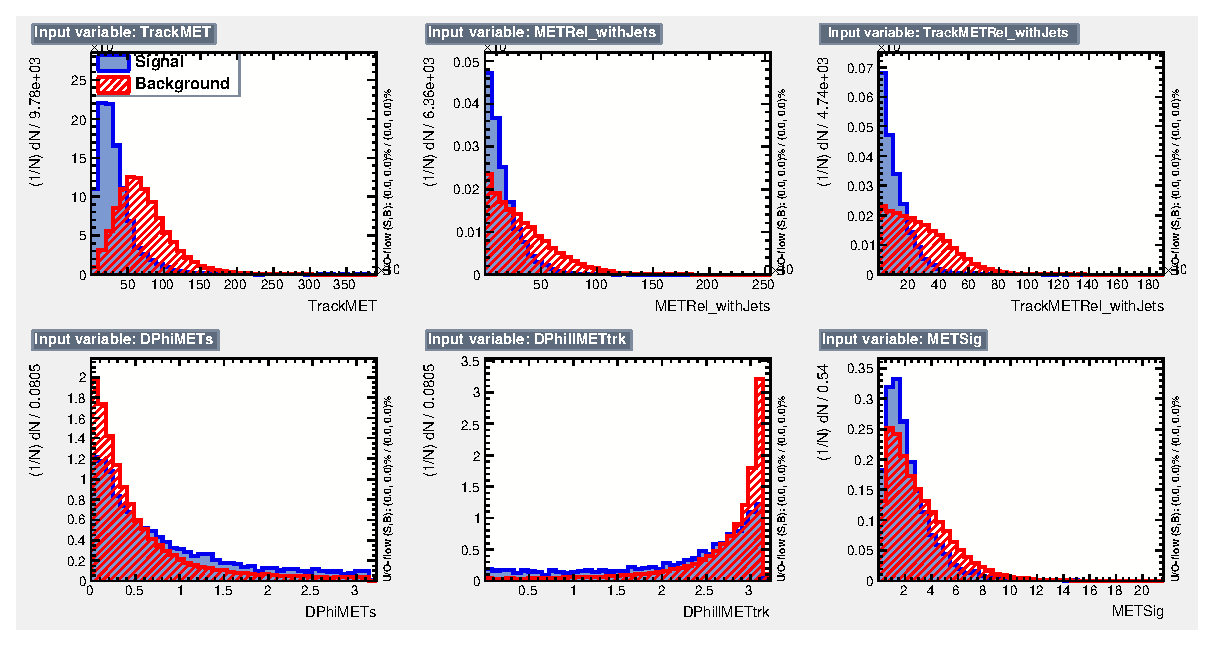
\includegraphics[width=0.85\linewidth]{Pictures/variables_id_c1.eps}
    \caption{Distributions of input variables to $Z\rightarrow\tau\tau$ BDT. Samples are unweighted and normalized to even numbers of background and signal events. Signal represents $Z\rightarrow\tau\tau$ and background VBF Higgs.}.
    \label{fig:ZjetsBDTinput}
\end{figure}
\begin{figure}[!htbp]
\centering
  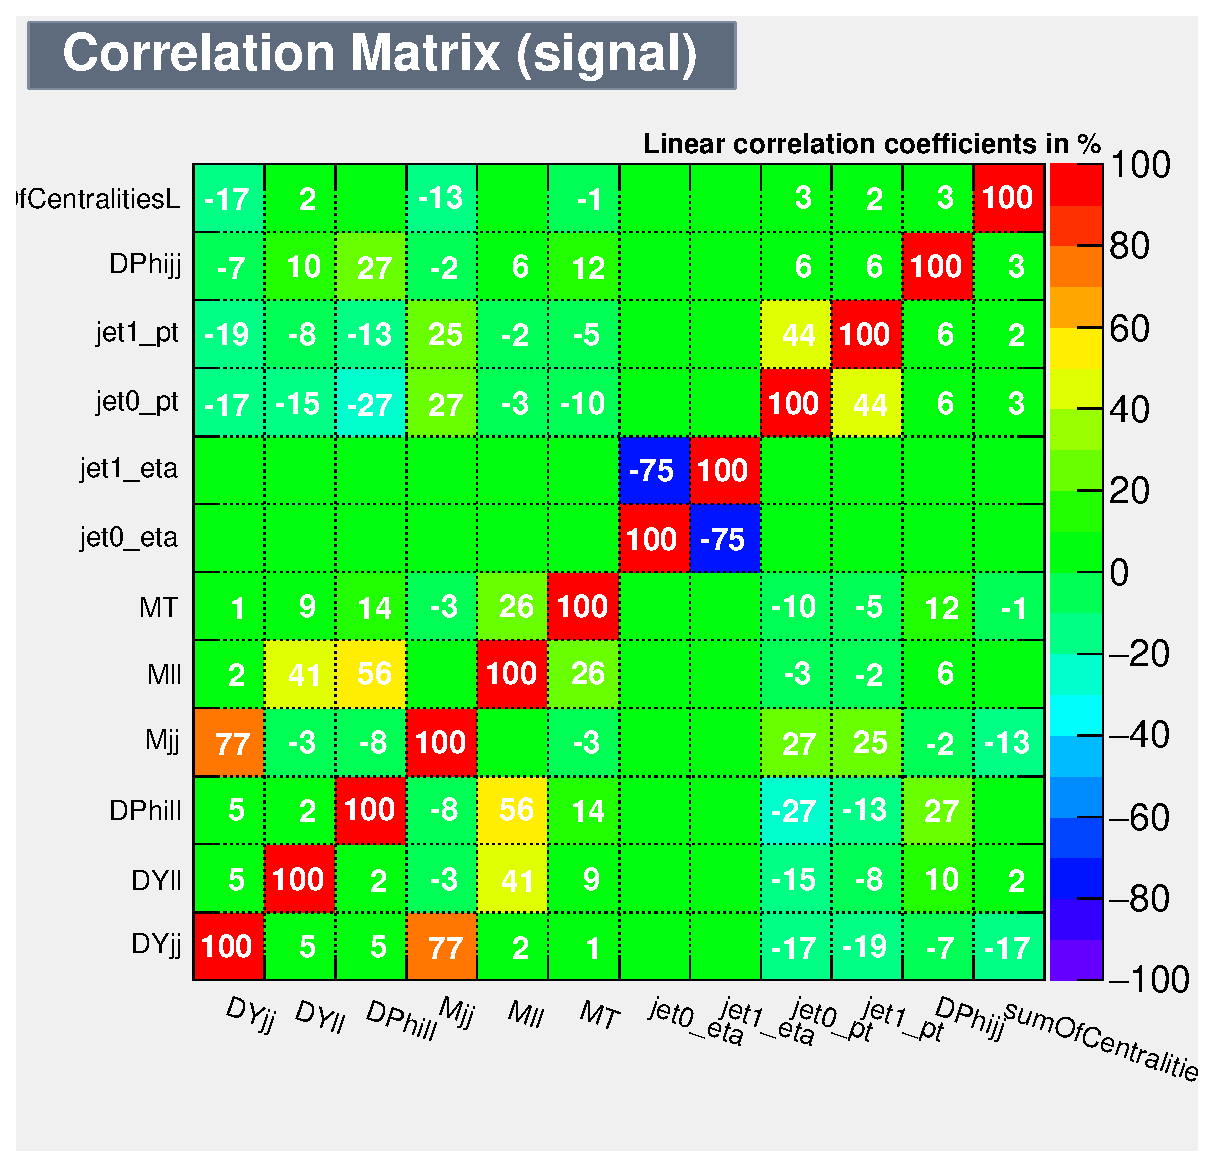
\includegraphics[width=.4\linewidth]{Pictures/CorrelationMatrixS.eps}
  \includegraphics[width=.4\linewidth]{Pictures/CorrelationMatrixB.eps}
\caption{Correlations of input variables to $Z\rightarrow\tau\tau$ BDT. Signal represents $Z\rightarrow\tau\tau$ and background VBF Higgs.}
\label{fig:ZjetscorrSB}
\end{figure}
The BDT training successfully separates $Z\rightarrow\tau\tau$ and VBF signal. In order to quantify the discrimination we use the integrated-ROC calculated through TMVA for unweighted normalized samples and find an optimal value of 0.897. Comparisons between the test and training show that the BDT is un-biased- differences between testing and training samples would imply overtraining, or the BDT using to many parameters on too few events. Visually, once can see that the testing and trainings samples are quite similar. Additionally, a Kolmogorov-Smirnov test is performed to measure if the two test and training distributions differ significantly. If the two distributions are random samples of the same parent distribution, the KS-test would give a uniformly distributed value between zero and one (or an average value of 0.5). The closer to 0.5 the KS-test, the greater likelihood the curves come from the same parent, however this calculation is heavily skewed toward lower values so any value above zero (or not very close to zero, on order $10^{-4}$) can be considered not indicative of overtraining. For signal and background we find KS-test values of 0.062 and 0.286, and so no evidence of over-training. We can visualize the BDT output variable both on un-weighted normalized samples and on samples with all event weights applied. The following plots show BDT results applied to un-weighted and weighted samples of $Z\rightarrow\tau\tau$ and VBF signal.

\begin{figure}[!htbp]
 \centering
  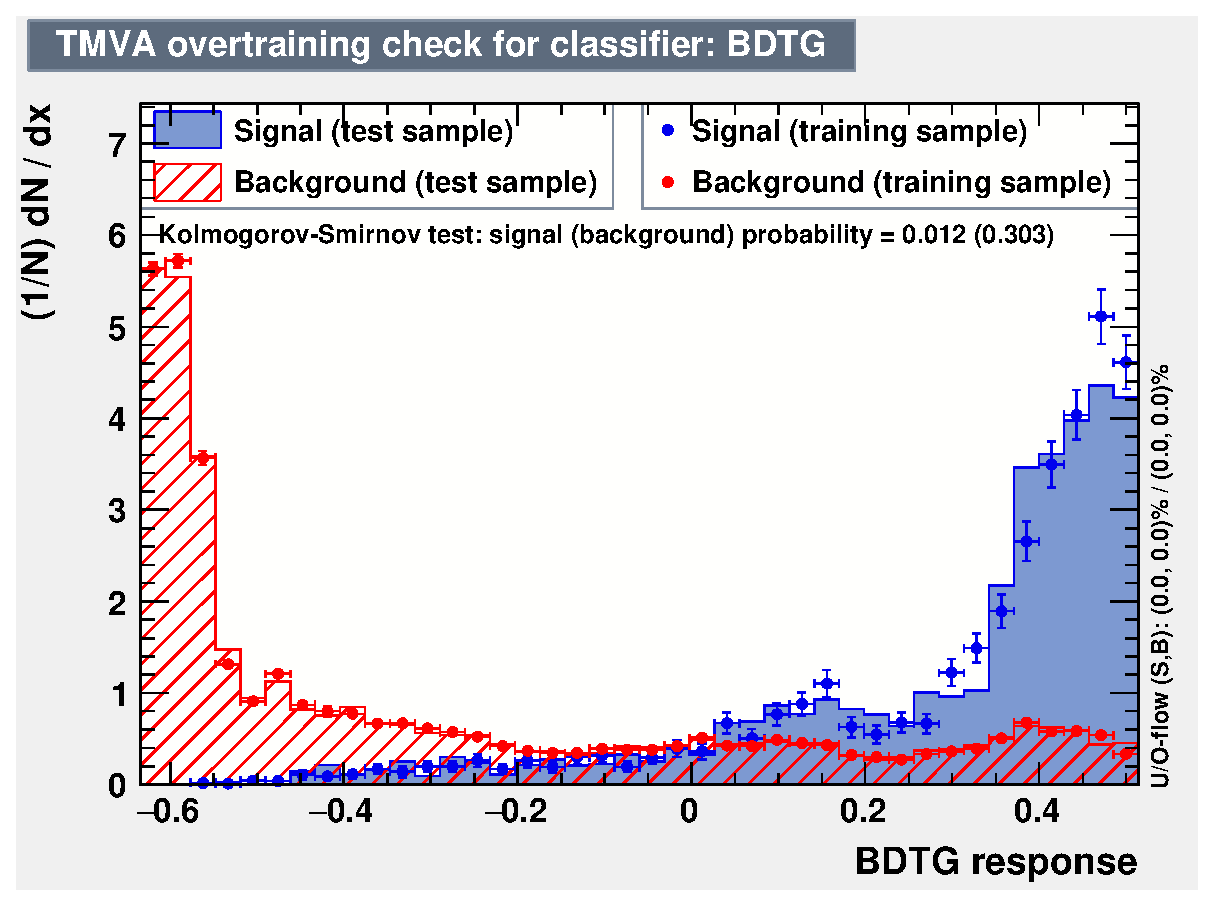
\includegraphics[width=.45\linewidth]{Pictures/ZttBDT/overtrain_BDTG.eps}
  \includegraphics[width=.35\linewidth]{Pictures/run2-emme-CutVBF_2jet-BDT_Zjets-log.pdf}
\caption{Unweighted, normalized samples of $\Ztt$ (signal) and VBF (background) plotted over BDT output distribution on left, overlaid testing and training samples shown. Right, full weighted samples of VBF signal, $\Ztt$, and all other backgrounds plotted over BDT output distribution after pre-selection cuts.}
\label{fig:ZjetsBDTresult}
\end{figure}

The plot \ref{fig:ZjetsBDTinterpret} shows distributions of all backgrounds as well as signal with $\Ztt$ BDT output in the signal region. Cuts on the BDT output variable are chosen to increase significance while also maintaining high signal statistics. Cutting on a BDT output value of 0.5, eliminates $60\%$ of $\Ztt$ background, or $\approx 450$ events, and only $6\%$ of signal events. This cut is also tested on truth samples to validate that applying it does not affect the fiducial phase space. 

\begin{figure}[!htbp]
\centering
\includegraphics[width=.6\linewidth]{Pictures/ZttBDT/run2-emme-CutVBF_ZttBDT-BDT_Zjets-log.pdf}
\caption{Full weighted samples of all signal and background plotted over BDT output distributions in SR after cut on $\Ztt$ BDT}
\label{fig:ZjetsBDTintepret}
\end{figure}

Four different iterations of signal and $\Ztt$ control region definitions are used in the simultaneous fit with Asimov data and overall results are examined with and without systematic uncertainties. The signal region is defined as described in the main text with at least 2 jets ($n_{jets}>=2$), a $b$-veto, $\Ztt$ veto, central-jet-veto (CJV), an outside-lepton-veto (OLV), and cuts on $m_{jj}>200$ GeV and on the rapidity difference between the two jets ($DY_{jj}>2.1$). The $\Ztt$ control region is defined in two different ways- first, as in the text with SR cuts requiring 2 jets, a b-veto, OLV and CJV as well as additional cuts reversing the $\Ztt$ veto with $66.2$~GeV $< m_{\tau\tau}< 116.2 $~GeV and an additional cut on $m_{ll}<80$~GeV. An alternative definition of the $\Ztt$ control region is within the signal region with orthogonality defined with a cut on the $\Ztt$ BDT. The four tested configurations are described in the table below. 

\begin{table}[h!]
\centering
\begin{tabular}{|l|c|c|c|}
\hline
Testing parameter name      & Signal region   & $\Ztt$ control region & $\Ztt$ control region axis     \\
\hline
\textbf{A}                           & default & $\Ztt$ CR & $m_T$  \\
\textbf{B}                           & default + $bdt_Zjets>0.5$ & $\Ztt$ CR & $m_T$    \\
\textbf{C}                           & Signal region + $bdt_{\Ztt}>0.5$ & Signal region + $bdt_{\Ztt}<0.5$ & $bdt_{\Ztt}$ \\
\textbf{D}			    & Signal region +$bdt_{\Ztt}>0.0$ & Signal region + $bdt_{\Ztt}<0.0$     & $bdt_{\Ztt}$\\
\hline
\end{tabular}
\caption{Four testing conditions defined for use in simultaneous fit}
\label{tab:ZBDTfitconditions}
\end{table}

The four testing conditions were included in a simultaneous fit with other regions defined with control regions and parameters as detailed in the main text. These studies are conducted with $v20$ pxAODS and associated $v20$ trained BDTs. First, stat-only results for each set of testing parameters are compiled in following table. 

\begin{table}[h!]
\centering
\begin{tabular}{|l|c|c|c|c|}
\hline
     & \textbf{A}   & \textbf{B} & \textbf{C} & \textbf{D}     \\
\hline
$\mu_{VBF}$ & $1 \pm 0.171$ &  $1 \pm 0.165$ & $1.00 \pm 0.143$ & $1.00 \pm 0.169$\\
$\mu_{\Ztt}$ & $1 \pm 0.00486$ & $0.999 \pm 0.038$ & $0.999 \pm 0.0197$ & $1.00\pm 0.052$\\
$\mu_{ggF}$ & $0.999 \pm 0.485$ & $1.00 \pm 0.451$ & $0.999 \pm 0.294$ & $0.999 \pm 0.469$\\
$\mu_{ggF1}$ & $1.00 \pm 0.449$ & $1.00 \pm 0.430$ & $1.00 \pm 0.269$ & $1.00 \pm 0.439$\\
$\mu_{ggF2}$ & $0.999 \pm 0.151$ & $1.00 \pm 0.172$ & $1.00 \pm 0.129$ & $0.999 \pm 0.172$\\
$\mu_{TopWW}$ & $1 \pm 0.0128$ & $1 \pm 0.014$ & $1 \pm 0.0033$ & $1 \pm 0.0096$ \\
\hline
\end{tabular}
\caption{Four testing conditions defined for use in simultaneous fit using only statistical uncertainties}
\label{tab:ZBDTstatonly}
\end{table}
 
These studies show no large gains from using conditions \textbf{B} or \textbf{D} instead of the default of \textbf{A} in which no BDT is used at all. Using condition \textbf{C} may have some positive effect from use of the BDT as both a binning cut to determine the $\Ztt$ background region within the signal region and VBF signal region itself and an axis used in the total fit. However adding systematics to this affects the overall results differently.  

\begin{table}[h!]
\centering
\begin{tabular}{|l|c|c|c|c|}
\hline
     & \textbf{A}   & \textbf{B} & \textbf{C} & \textbf{D}     \\
\hline
$\mu_{VBF}$ & $1 \pm 0.202$ &  $1 \pm 0.196$ & $1.00 \pm 0.196$ & $1.00 \pm 0.195$\\
$\mu_{\Ztt}$ & $1 \pm 0.0185$ & $0.999 \pm 0.056$ & $0.999 \pm 0.0536$ & $1.00\pm 0.0759$\\
$\mu_{ggF}$ & $0.999 \pm 0.645$ & $1.00 \pm 0.646$ & $0.999 \pm 0.648$ & $0.999 \pm 0.670$\\
$\mu_{ggF1}$ & $1.00 \pm 0.565$ & $1.00 \pm 0.566$ & $1.00 \pm 0.574$ & $1.00 \pm 0.587$\\
$\mu_{ggF2}$ & $0.999 \pm 0.407$ & $1.00 \pm 0.323$ & $1.00 \pm 0.323$ & $0.999 \pm 0.272$\\
$\mu_{TopWW}$ & $1 \pm 0.0184$ & $1 \pm 0.017$ & $1 \pm 0.0176$ & $1 \pm 0.0154$ \\
\hline
\end{tabular}
\caption{Four testing conditions defined for use in simultaneous fit using and systematic and statistical uncertainties}
\label{tab:ZBDTstatsys}
\end{table}

Overall results are not changed significantly by the addition of the $BDT_{\Ztt}$ parameter in the overall fit when systematic uncertainties are taken into account. The low statistics of $\Ztt$ events in its designated control region (within or outside the signal region) likely cause the higher uncertainties when this cut is used. After the conclusion of these studies configuration \textbf{A} was chosen for the analysis. 

The plots following show results from the each iteration- first correlation plots then plots showing the $\Ztt$, WW and top regions after each type of fit.
\begin{figure}[!htbp]
\centering
\includegraphics[width=.9\linewidth]{Pictures/ZttBDT/correlations.png}
\caption{Correlations on fit parameters for each of four region parameters}
\label{fig:ZjetsBDTcorrelation}
\end{figure} 

\begin{figure}[!htbp]
\centering
\includegraphics[width=.9\linewidth]{Pictures/ZttBDT/ZttCR.png}
\caption{$\Ztt$ distributions for each of four region parameters}
\label{fig:ZjetsBDTZttCR}
\end{figure} 

\begin{figure}[!htbp]
\centering
\includegraphics[width=.9\linewidth]{Pictures/ZttBDT/TopWWCR.png}
\caption{Top and WW distributions for each of four region parameters}
\label{fig:ZjetsBDTTopWWCR}
\end{figure} 

%\begin{figure}[!htbp]
%\centering
  %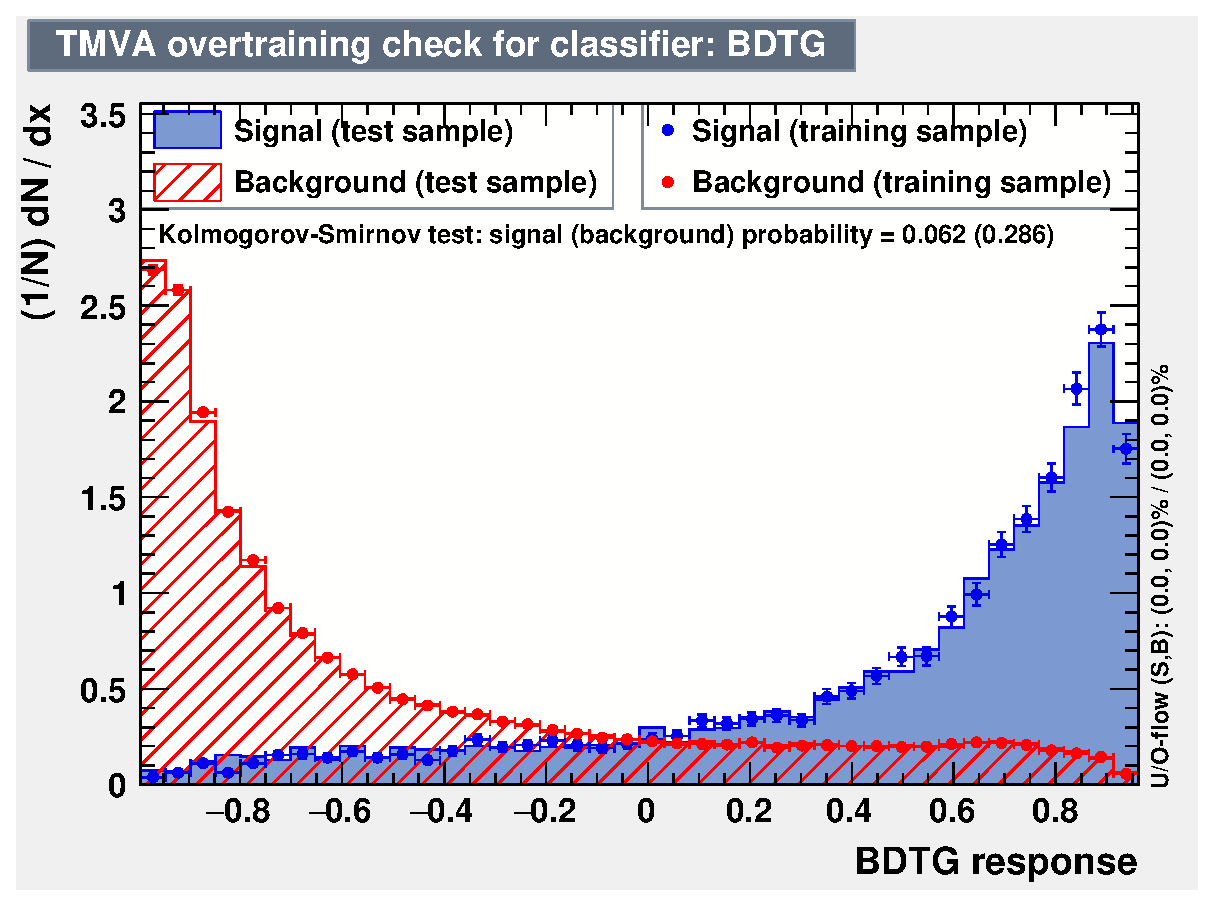
\includegraphics[width=.4\linewidth]{Pictures/overtrain_BDTG.eps}
%  \includegraphics[width=.4\linewidth]{Pictures/weightedZjetsVBF.png}
%\caption{Weighted, normalized samples of $Z\rightarrow\tau\tau$ (signal) and VBF (background) plotted over BDT output distribution on left, overlaid testing and training samples shown. On right, full weighted samples of $Z\rightarrow\tau\tau$ and VBF signal plotted over BDT output distributions.}
%\label{fig:ZjetsBDTresult}
%\end{figure}

%Finally, we can test how other background samples distribute with the $Z\rightarrow\tau\tau$ BDT output variable and optimize results from cutting on this variable. The following plot \ref{fig:ZjetsBDTinterpret} shows distribution of all backgrounds as well as signal with $Z\rightarrow\tau\tau$ BDT output. We aim to increase significance while also keeping as much signal sample as possible for keep high statistics. To accomplish this we cut at a BDT output value of 0.5, in this way we eliminate $60\%$ of $Z\rightarrow\tau\tau$ background, or $\approx 450$events, and only $6\%$ of signal events. We have also tested this cut on truth samples to validate that applying this cut does not affect our fiducial phase space. 
%\begin{figure}[!htbp]
%\centering
%\includegraphics[width=.4\linewidth]{Pictures/weightedZjetsAll.png}
%\caption{Full weighted samples of all signal and background plotted over BDT output distributions}
%\label{fig:ZjetsBDTintepret}
%\end{figure}

%The BDT that discriminates VBF signal and $Z+$jets is applied in the $Z+$jets control region to maintain orthogonality. This further increases purity in the control region. This distribution is shown in the following plot.
%\begin{figure}[!htbp]
%\centering
%\includegraphics[width=.6\linewidth]{Pictures/run2-emme-CutVBFZtautauControl_2jetinclBDT-BDT_Zjets-log.pdf}
%\caption{Full weighted samples of all signal and background plotted over BDT output distributions in $Z+$jets control region after cut on $Z+$jets BDT}
%\label{fig:ZjetsBDTCR}
%\end{figure}


